%!TEX root = ../dokumentation.tex

\chapter{\label{sec:parsen}Parsen und Datenstruktur}
Der erste Schritt zum automatischen Beweisen eines Tableau, ist das Parsen der String-Repräsentation zu einer vom Programm weiterverarbeitbaren Datenstruktur. Hierfür wird im folgenden zuerst die Syntax definiert, in der die Formeln als Zeichenkette dargestellt werden. Danach wird die Datenstruktur, in der die Formel weiterverarbeitet wird, besprochen. Zuletzt wird der Parser und die Implementierung dessen behandelt.

\section{\label{sec:syntaxdef}Syntaxdefinition}
Prinzipiell wurde die Syntax in der die Formeln als String repräsentiert werden bereits in \autoref{sec:ind_form_regeln} beschrieben. Da die Buchstaben zur Darstellung der Operatoren aber auf handelsüblichen Tastaturen nicht vorhanden sind, müssen hierfür benutzerfreundlichere Alternativen definiert werden. Da die Zielgruppe des Tableaubeweisers meist schon mit Programmiersprachen in Berührung gekommen ist, wird sich dabei an den in Programmiersprachen üblichen Buchstaben orientiert. So wird z.B. für das Oder ($\vee$) das in Java, C\#, Swift und weiteren verwendete | definiert (in diesen Sprachen steht das einfache | für ein Bitweises-Oder, in diesem Fall gibt es allerdings keine Integer-Werte was eine Unterscheidung sinnlos macht).

Die vollständige Definition der insgesamt 7 Operatoren zu ihren tastaturfreundlichen Gegenspielern wird in \autoref{tbl:operator_mapping} aufgeführt.
\begin{table}[h]
\begin{center}
\begin{tabular}{|c|c|c|c|}
\hline
Operator-Symbol & Tastaturfreundliches Symbol & Alternatives Symbol \\
\hline
$\forall$ & (A) & /\textbackslash \\
\hline
$\exists$ & (E) & \textbackslash/ \\
\hline
$\neg$ & ! & - \\
\hline
$\wedge$ & \& & * \\
\hline
$\vee$ & | & + \\
\hline
$\rightarrow$ & -> & \\
\hline
$\leftrightarrow$ & <-> & \\
\hline
\end{tabular}
\end{center}
\caption{\label{tbl:operator_mapping}Definition der tastaturfreundlichen Operator-Symbole}
\end{table}

Zur Darstellung für Klammern werden nach wie vor die Runden Klammern ( und ) verwendet.

Ebenfalls zur Definition der Syntax gehört es zu definieren in welcher Form die atomaren Aussagen sowie Variablen, Konstanten und Funktionen in der Prädikatenlogik angegeben werden. Da es in der klassischen sowie nichtklassischen Aussagenlogik kein Risiko für Ambiguitäten zwischen Funktion und Prädikat oder ähnlichem gibt, dürfen diese mit Klein- und Großbuchstaben beginnen. Zudem darf die atomare Aussage Zahlen und Unterstriche enthalten, muss aber mit einem Buchstaben beginnen.

Bei der klassischen und nichtklassischen Prädikatenlogik kann es allerdings zu besagten Ambiguitäten kommen. Um bereits an der Schreibweise zu klären, um was es sich handelt werden hier folgende Regeln eingeführt:
\begin{itemize}
\item \textbf{Prädikat}: Ein Prädikat muss mit einem Großbuchstaben beginnen. Danach kann dieses beliebe Klein- und Großbuchstaben sowie Zahlen und Unterstriche enthalten.

\item \textbf{Funktion}: Ein Prädikat muss mit einem Kleinbuchstaben beginnen. Danach kann dieses beliebe Klein- und Großbuchstaben sowie Zahlen und Unterstriche enthalten.

\item \textbf{Konstante}: Eine Konstante muss mit einem Großbuchstaben beginnen. Danach kann dieses beliebe Klein- und Großbuchstaben sowie Zahlen enthalten.

\item \textbf{Variable}: Eine Variable muss mit einem Kleinbuchstaben beginnen. Danach kann dieses beliebe Klein- und Großbuchstaben sowie Zahlen enthalten.
\end{itemize}

Man beachte, dass Konstanten und Variablen keine Unterstriche enthalten dürfen. Dies liegt daran, dass während des automatischen Beweisens von prädikatenlogischen Aussagen unter Umständen neue Konstanten eingeführt werden. Um keine Analyse der existierenden Konstanten durchführen zu müssen, um zu berechne,n welche Konstanten noch nicht eingeführt sind, wird das Unterstrich-Zeichen für diese Konstanten reserviert. Eine dadurch eingeführte Konstante wird dann als ``X\_n'' eingeführt, wobei n der fortlaufende Index der eingeführten Konstante ist.


\section{Datenstruktur}
Mit einer Formel in der oben definierten Syntax kann nicht direkt weitergearbeitet werden. Um dies zu tun, muss diese in einer Datenstruktur vorliegen, mit der ein Computer sinnvoll rechnen kann.
Deshalb wird diese in einen Syntaxbaum geparsed. In einem Syntaxbaum stellt jeder innere Knoten einen Operator und jeder Kind-Knoten einen Operanden der Operatoren. \cite{compiler_dragon_book} In diesem Fall wären die Kind-Knoten die atomaren Aussagen. Ein Beispiel eines solchen Syntaxbaums für die Aussage A$\vee$B$\rightarrow\neg$C ist in \autoref{fig:example_syntax_tree} dargestellt.

\begin{figure}[H]
\begin{center}
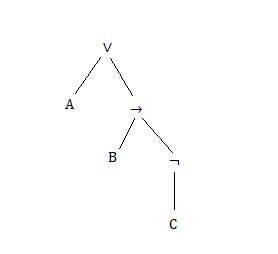
\includegraphics[scale=1]{images/example_syntax_tree.png}
\caption{Beispiel eines Syntaxbaumes der Aussage A$\vee$B$\rightarrow\neg$C}
\label{fig:example_syntax_tree}
\end{center}
\end{figure}

Das Konzept eines Syntaxbaums übersetzt in die für diese Arbeit verwendete objektorientierte Programmiersprache Python, ergibt eine Datenstruktur, in der die einzelnen Operatoren und atomaren Aussagen Objekten entsprechen, die jeweils ihre Kind-Knoten als Variablen halten. Das Klassendiagramm für die Aussagenlogik ist in \autoref{fig:class_diag_ds_pl} zu sehen.

\begin{figure}[H]
\begin{center}
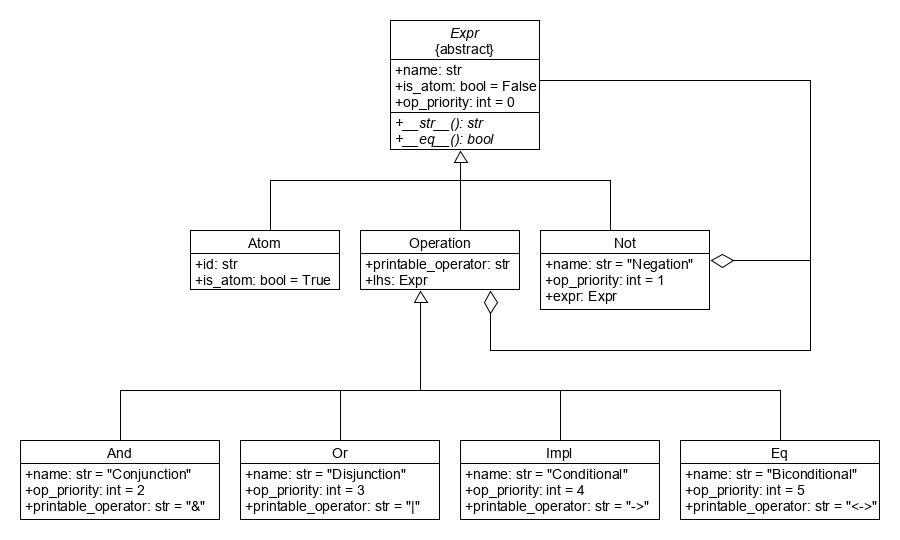
\includegraphics[scale=0.5]{images/class_diag_ds_pl.png}
\caption{Klassendiagramm der Aussagenlogik}
\label{fig:class_diag_ds_pl}
\end{center}
\end{figure}

Der Syntaxbaum für die Prädikatenlogik sieht mehr oder weniger ähnlich aus. Der große Unterschied hierbei ist die atomare Aussage. Diese ist in der Prädikatenlogik die Klasse \textit{Predicate} wobei diese eine Liste von Termen, also Funktionen, Konstanten und Variablen hält. Zudem gibt es die beiden weiteren Quantifikatoren-Klassen. Der Ausschnitt aus dem Klassendiagramm mit den zusätzlichen Klassen ist in \autoref{fig:class_diag_ds_fopl} dargestellt.

\begin{figure}[H]
\begin{center}
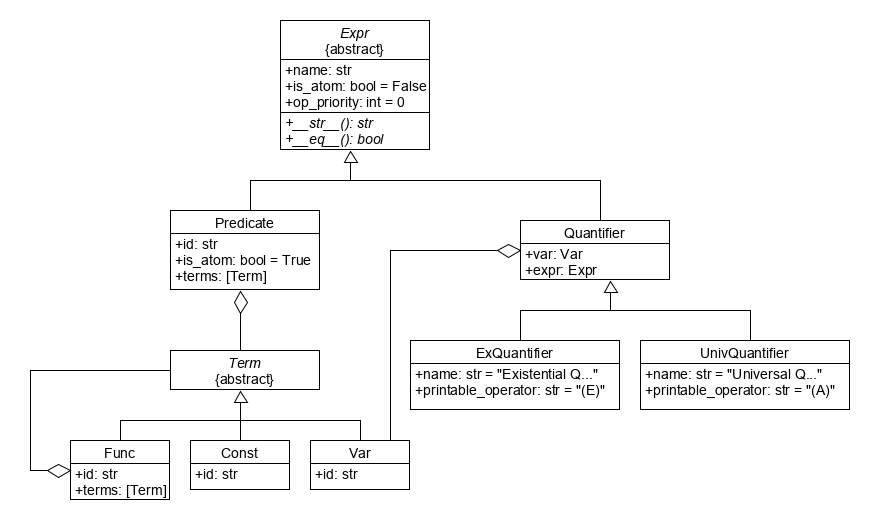
\includegraphics[scale=0.5]{images/class_diag_ds_fopl.png}
\caption{Ausschnitt des Klassendiagramm der Prädikatenlogik}
\label{fig:class_diag_ds_fopl}
\end{center}
\end{figure}

In der definierten Datenstruktur sieht der in \autoref{fig:example_syntax_tree} dargestellte Syntaxbaum also wie im Objektdiagramm in \autoref{fig:obj_diag_syn_tree} zu sehen aus.

\begin{figure}[H]
\begin{center}
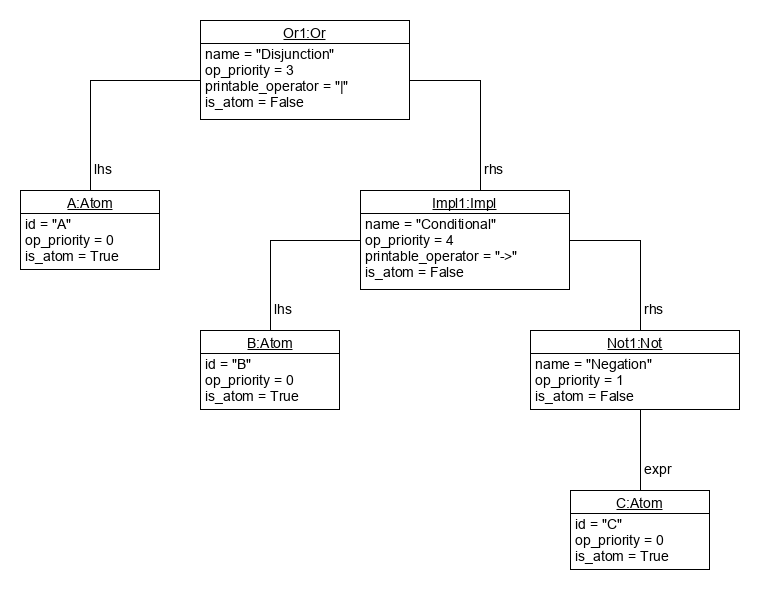
\includegraphics[scale=0.5]{images/obj_diag_syn_tree.png}
\caption{Objektdiagramm des Syntaxbaums der Aussage A$\vee$B$\rightarrow\neg$C}
\label{fig:obj_diag_syn_tree}
\end{center}
\end{figure}


\section{Parsen}
Da nun klar ist, wie die Syntax und Datenstruktur der Formeln aussieht, muss noch die Zeichenketten-Repräsentation zur Datenstruktur geparsed werden.

Zum Erstellen des Parsers, wird der Parsergenerator ANTLR verwendet. Mit ANTLR kann eine Grammatik definiert werden, von der dann ein LL(*)-Parser in einer von vielen möglichen Programmiersprachen generiert wird. Generiert werden kann unter anderem Java, C\#, JavaScript aber auch Python. \cite{antlr_doc}

\subsection{LL(*)-Parser}
Im Gegensatz zu dem vorherrschenden Bottom-Up Parsertyp LR(k), wird für von ANTLR generierte Parser ein Top-Down Parser erzeugt. \cite{compiler_dragon_book}\cite{ll_star_parser}

Der hierfür verwendete Parsertyp LL(*) wurde eigens für ANTLR entwickelt. LL steht dafür, dass die Eingabe von links nach rechts gelesen und eine Linksableitung davon gebildet wird. Der Stern bedeutet, dass bei jedem Schritt für Parsing-Entscheidungen beliebig viele Eingabesymbole vorausgeschaut wird. \cite{ll_star_parser} Im Gegensatz dazu wird beim Parsertyp LR(k), bei dem das L ebenfalls für das Lesen der Eingabe von links nach rechts steht, das R für das Erstellen einer umgekehrten Rechtsableitung und das k dafür wie viele Zeichen nach vorn geschaut wird. Die Vorausschau wird also durch k gedeckelt. \cite{compiler_dragon_book}

Mit LL(*) werden von ANTLR prädikative Grammatiken geparsed. Eine prädikative Grammatik G ist ein 6-Tupel (N, T, P, S, $\Pi$, M). Die Elemente haben folgende Bedeutung \cite{ll_star_parser}:
\begin{itemize}
\item \textbf{N}: N ist eine endliche Menge von Nichtterminalen, also Variablen die mittels Produktionsregeln in P auf weitere Nichtterminale bzw. Terminale abgeleitet werden können.

\item \textbf{T}: T ist eine endliche Menge von Terminalen, also Ausdrücken die nicht weiter abgeleitet werden können. Diese Menge wird oft auch als Alphabet der Sprache von G bezeichnet.

\item \textbf{P}: P ist eine endliche Relation von V nach (V$\cup\Sigma$)*, wobei der * den kleenschen Hüllenoperator bedeutet (siehe Unten). Zudem sind mit Prädikaten bedingte Produktionen und Mutatoren als Produktionsregeln möglich. Eine mit Prädikat $\pi_{i}\in\Pi$ bedingte Produktion kann angewandt werden gdw. $\pi_{i}$ wahr ist. Ein Mutator $\mu_{i}\in$M ist wird mit einem Zustand aufgerufen und gibt einen neuen Zustand zurück.

\item \textbf{S}: S$\in$N definiert das Startsymbol von dem aus alle Sätze der Sprache mittels der Produktionsregeln in P abgeleitet werden können.

\item \textbf{$\Pi$}: $\Pi$ definiert semantische Prädikate. Ein solches Prädikat wird in der Zielsprache (z.B. Python) in der Grammatik angegeben. Das Prädikat nimmt den aktuellen Parse-Zustand als Eingabe und gibt einen Wahrheitswert zurück.

\item \textbf{M}: M definiert eine Menge von Aktionen oder Mutatoren. Diese werden in der Zielsprache in der Grammatik angegeben. Dieser nimmt den Parse-Zustand als Eingabe und gibt einen neuen Zustand zurück.
\end{itemize}

Die kleensche Hülle $\Sigma$* einer Menge $\Sigma$ ist wie folgt definiert. $\epsilon\in\Sigma$*, wobei $\epsilon$ das leere Wort repräsentiert. Zudem gilt $\forall$w,a (w$\in\Sigma$*)$\vee$(a$\in\Sigma$)$\rightarrow$wa$\in\Sigma$*. \cite{compiler_dragon_book}

Für die hier behandelten Zwecke wird der Sprachumfang der prädikativen Grammatiken nicht benötigt. Es genügt die kontextfreie Grammatik zu betrachten wobei $\Pi$ und M wegfällt.

Eine Beispiel Grammatik G = (N, T, P, Expr) wäre folgende: \\
N = \{Expr, Id\} \\
$\Sigma$ = \{a, b, +, -\} \\
P = \{Expr$\rightarrow$Expr+Expr, Expr$\rightarrow$Expr-Expr, Expr$\rightarrow$Id, Id$\rightarrow$a, Id$\rightarrow$b\} \\

Aus dieser Grammatik könnten unter anderem folgende Sätze abgeleitet werden: a+b, a+b-a, a+a+a, ...

Die schwierige Herausforderung eines Parsers ist es nun zu entscheiden, ob eine gegebene Zeichenfolge mit der Grammatik erzeugbar ist und mit welchen Terminalen diese aufgebaut ist. Insbesondere wird dies schwierig, sind Terminale mit ähnlichem Präfix vorhanden wie z.B.: ab und abb. Der Parser muss hierbei in der Zeichenkette also bis zu 3 Zeichen untersuchen bis er entscheiden kann zu welchem der beiden Terminale diese zugeordnet werden kann.

LL(*) erzeugt hierfür einen \ac{DEA} für jede Ableitungsregel. Der \ac{DEA} wechselt für jedes Zeichen bzw. für jedes Terminal den Zustand wodurch die zutreffende Ableitungsregel am Ende der Zeichenkette erreicht ist. Eine Ausnahme hierfür sind Rekursiv definierte Regeln, wie die obige, für das Nichtterminal Expr. Diese leitet wieder auf das Nichtterminal Expr ab. Für solche Regeln, wird ein \ac{DEA} für die ersten m Rekursionsebenen erzeugt, ist danach noch keine eindeutige Ableitung erreicht, wird mittels Backtracking der Rest der Zeichenkette analysiert.
Die beliebig weite Vorausschau ergibt sich eben durch das Backtracking, aber auch durch die Definition von Terminalen durch reguläre Ausdrücke. Um welches Terminal es sich handelt, wird durch Abgleich aller regulärer Ausdrücke entschieden, wobei bei mehreren Treffern das zuerst definierte Terminal gewinnt. \cite{ll_star_parser}

Top-Down Parser können Grammatiken die eine Linksrekursion enthalten generell nicht handhaben. \cite{compiler_dragon_book} Eine Grammatik enthält eine Linksrekursion, gdw. sie eine Ableitung der Form A$\xrightarrow{\text{+}}$A$\alpha$ enthält, wobei $\xrightarrow{\text{+}}$ bedeutet, dass die Ableitung über beliebig viele andere Ableitungen zu A$\alpha$ abgeleitet werden kann.
Eine solche Ableitungsregel gilt es deshalb in der Grammatikdefinition zu vermeiden.

\subsection{ANTLR-Grammatiken}
Eine ANTLR-Grammatik ist relativ simpel aufgebaut. Nichtterminale werden in Kleinbuchstaben geschrieben, während Terminale in Großbuchstaben geschrieben werden. Wichtig ist es, dass zur Vermeidung von Grammatiken, die einen Satz über mehrere Ableitungsfolgen erzeugen können, die Ableitungsregeln, die zuerst definiert werden eine höhere Priorität gegenüber später definierten haben. \cite{antlr_doc}
Dieser Umstand kann auch zur Abbildung der Prioritäten von Operatoren genutzt werden.

Kann ein Nichtterminal mit mehreren Produktionsregeln abgeleitet werden, so können diese mit ``|'' getrennt aufgelistet werden. Ein Terminal kann wie oben bereits erwähnt, durch reguläre Ausdrücke definiert werden.

\subsection{Grammatikdefinition}
Nun muss aus in \autoref{sec:syntaxdef} definierter Syntax eine ANTLR-Grammatik definiert werden.

Die Grammatik für Aussagenlogik ist relativ simpel und in \autoref{lst:grammatik_aussagenlogik} zu sehen.

\begin{lstlisting}[caption={Grammatik der Aussagenlogik},label=lst:grammatik_aussagenlogik]
expr :
	ATOM |
	NOT expr |
	expr AND expr |
	expr OR expr |
	expr IMPL expr |
	expr EQ expr |
	OPENCLAMP expr CLOSECLAMP;

ATOM : [A-Za-z0-9]+;

OR : '|' | '+';
AND : '&' | '*';
IMPL : '->';
NOT : '!' | '-';
EQ : '<->';
OPENCLAMP : '(';
CLOSECLAMP : ')';
\end{lstlisting}

Da die Grammatik der Prädikatenlogik zusätzlich Prädikate und Funktionen beliebiger Stelligkeit abbilden muss, ist diese etwas komplexer. Die Grammatik ist in \autoref{lst:grammatik_prädlogik} zu sehen.

\begin{lstlisting}[caption={Grammatik der Prädikatenlogik},label=lst:grammatik_prädlogik]
expr :
    predicate |
    quantor expr |
    NOT expr |
    expr AND expr |
    expr OR expr |
    expr IMPL expr |
    expr EQ expr |
    OPENCLAMP expr CLOSECLAMP;

predicate : PREDNAME (terms |) CLOSECLAMP;

quantor : (ALL_QUANTOR | EX_QUANTOR) var varlist;

terms : term termlist;
termlist : COMMA term termlist | ;
term : var | const | func;

var : VARNAME;
const : CONSTNAME;
varlist : COMMA var varlist |;

func : FUNCNAME (terms |) CLOSECLAMP;

PREDNAME : [A-Z][A-Za-z0-9_]*'(';
VARNAME : [a-z][A-Za-z0-9]*;
CONSTNAME : [A-Z][A-Za-z0-9]*;
FUNCNAME : [a-z][A-Za-z0-9_]*'(';

OR : '|' | '+';
AND : '&' | '*';
IMPL : '->';
NOT : '!' | '-';
EQ : '<->';
OPENCLAMP : '(';
CLOSECLAMP : ')';
COMMA : ',';

ALL_QUANTOR : '(A)' | '/\';
EX_QUANTOR : '(E)' | '\/';
\end{lstlisting}